
\subsection{Nghiên cứu và lựa chọn các công cụ hỗ trợ quản lý dự án}
Trong quy trình Scrum, việc quản lý mã nguồn và tiến độ là bắt buộc. Do đó nhóm đã chọn các công cụ phổ biến sau.
\subsubsection{Discord}
    \begin{figure} [H]
        \centering
        
\includegraphics[width=0.4\linewidth]{3.Nghiên cứu//Images/Discord.png}
        % \caption{Discord}
        \label{fig:placeholder}
    \end{figure}
    Discord là một nền tảng giao tiếp trực tuyến được sử dụng rộng rãi trong lĩnh vực công nghệ thông tin nói chung và lập trình game nói riêng. Trong quá trình thực hiện dự án, Discord đóng vai trò là công cụ hỗ trợ chính cho việc quản lý nhóm, trao đổi kỹ thuật và phối hợp công việc giữa các thành viên. Nhóm sử dụng Discord để tổ chức các buổi họp trực tuyến, thảo luận về hướng phát triển game cũng như xử lý các vấn đề phát sinh trong quá trình làm.\\
    
    Discord cho phép tạo nhiều kênh thảo luận khác nhau theo từng mục đích cụ thể như trao đổi chung, lập trình, thiết kế gameplay và báo lỗi. Việc phân chia kênh giúp nội dung trao đổi được sắp xếp khoa học, tránh chồng chéo thông tin và nâng cao hiệu quả làm việc nhóm. Bên cạnh đó, Discord còn hỗ trợ chia sẻ nhanh các tài nguyên như mã nguồn, hình ảnh, video minh họa gameplay và các tài liệu thiết kế.\\

    Ngoài ra, nền tảng này còn hỗ trợ lưu trữ lịch sử trò chuyện, giúp các thành viên dễ dàng theo dõi lại quá trình thảo luận và quyết định kỹ thuật đã được thống nhất trước đó. Nhờ các tính năng trên, Discord góp phần nâng cao khả năng phối hợp, giảm thời gian trao đổi và hỗ trợ hiệu quả cho việc quản lý và phát triển dự án theo mô hình Scrum.

\subsubsection{Git}
\begin{figure} [H]
    \centering
    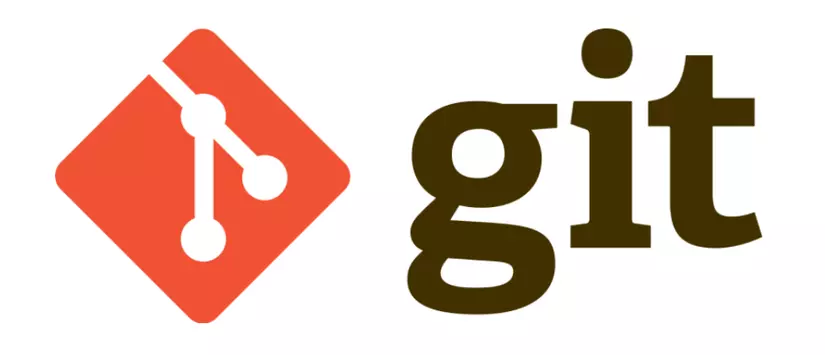
\includegraphics[width=0.4\linewidth]{3.Nghiên cứu//Images/Git.png}
    % \caption{Git}
    \label{fig:placeholder}
\end{figure}
    Git là một hệ thống quản lý phiên bản phân tán mã nguồn mở, được Linus Torvalds phát triển vào năm 2005 nhằm đáp ứng nhu cầu quản lý mã nguồn hiệu quả trong quá trình phát triển nhân hệ điều hành Linux. Cho đến nay, Git đã trở thành một trong những hệ thống quản lý phiên bản phổ biến và được sử dụng rộng rãi nhất trong lĩnh vực phát triển phần mềm. Git cho phép theo dõi toàn bộ lịch sử thay đổi của mã nguồn và hỗ trợ nhiều người làm việc đồng thời trên cùng một dự án.\\

    Một trong những ưu điểm nổi bật của Git là tốc độ xử lý nhanh, khả năng hoạt động ổn định ngay cả với các dự án có quy mô lớn. Git có giao diện dòng lệnh đơn giản, giúp các thành viên trong nhóm dễ dàng tiếp cận và sử dụng. Với đặc tính phân tán hoàn toàn, mỗi thành viên đều sở hữu một bản sao đầy đủ của mã nguồn trên máy cục bộ, cho phép làm việc ngoại tuyến và đồng bộ dữ liệu linh hoạt với các thành viên khác trong nhóm.\\

    Ngoài ra, Git hỗ trợ mạnh mẽ cho việc phát triển song song thông qua cơ chế nhánh (branch), giúp nhiều người có thể phát triển các chức năng khác nhau cùng lúc mà không ảnh hưởng trực tiếp đến mã nguồn chính. Git còn sử dụng các hàm băm mật mã để đảm bảo tính toàn vẹn của dữ liệu, giúp phát hiện nhanh chóng các thay đổi không hợp lệ hoặc sai sót trong quá trình chỉnh sửa mã nguồn. Nhờ những ưu điểm trên, Git đóng vai trò quan trọng trong việc quản lý mã nguồn hiệu quả cho dự án của nhóm.

\subsubsection{Github}
\begin{figure} [H]
    \centering
    
\includegraphics[width=0.4\linewidth]{3.Nghiên cứu//Images/Github.png}
    % \caption{Github}
    \label{fig:placeholder}
\end{figure}
GitHub là một nền tảng lưu trữ và quản lý mã nguồn trực tuyến dựa trên hệ thống quản lý phiên bản Git, được sử dụng rộng rãi trong cộng đồng phát triển phần mềm. Trong quá trình thực hiện dự án, GitHub được nhóm sử dụng để lưu trữ mã nguồn, đồng bộ dữ liệu giữa các thành viên và quản lý tiến độ phát triển dự án.\\

GitHub hỗ trợ làm việc nhóm thông qua các chức năng như kho lưu trữ (repository), nhánh (branch), gộp mã (merge) và yêu cầu hợp nhất (pull request). Nhờ đó, các thành viên có thể phát triển song song các chức năng khác nhau mà không gây ảnh hưởng trực tiếp đến mã nguồn chính. Ngoài ra, GitHub còn cung cấp hệ thống theo dõi lỗi (Issues), giúp ghi lại các lỗi phát sinh và phân công nhiệm vụ cho từng thành viên một cách rõ ràng.\\

Bên cạnh đó, GitHub còn lưu trữ đầy đủ lịch sử thay đổi của mã nguồn, giúp dễ dàng kiểm tra, khôi phục các phiên bản trước khi cần thiết. Nhờ những tính năng trên, GitHub đóng vai trò quan trọng trong việc quản lý mã nguồn, hỗ trợ làm việc nhóm hiệu quả và đảm bảo tính an toàn cho dự án của nhóm.

\subsubsection{Jira}
\begin{figure} [H]
    \centering
    
\includegraphics[width=0.4\linewidth]{3.Nghiên cứu//Images/Jira.png}
    % \caption{Jira}
    \label{fig:placeholder}
\end{figure}
Jira là một công cụ quản lý dự án và theo dõi tiến độ công việc do công ty Atlassian phát triển, được sử dụng phổ biến trong các dự án phát triển phần mềm theo mô hình Agile và Scrum. Trong quá trình thực hiện dự án của nhóm, Jira được nhóm sử dụng để quản lý công việc, theo dõi tiến độ từng giai đoạn và kiểm soát hiệu quả làm việc của các thành viên.\\

Jira cho phép tạo và quản lý các đầu việc (Issue) như Task, Bug, Story, từ đó phân công nhiệm vụ cụ thể cho từng thành viên trong nhóm. Mỗi công việc đều có trạng thái rõ ràng như ``To Do'', ``In Progress'', ``Done'', giúp nhóm dễ dàng theo dõi tiến độ thực hiện. Bên cạnh đó, Jira còn hỗ trợ xây dựng bảng Scrum, lập kế hoạch Sprint và theo dõi khối lượng công việc trong từng Sprint một cách trực quan.\\

Ngoài ra, Jira còn cung cấp các công cụ thống kê và báo cáo tiến độ như biểu đồ Burndown Chart, Velocity Chart, giúp nhóm đánh giá hiệu suất làm việc theo từng giai đoạn. Nhờ những tính năng trên, Jira hỗ trợ hiệu quả cho việc quản lý tiến độ, phân công nhiệm vụ và kiểm soát chất lượng dự án theo mô hình Scrum.
